% !TeX spellcheck = en_US
% !TeX encoding = UTF-8
% !TeX root = ../report.tex

\chapter{Simulation of the Bridgestone World Solar Challenge}
\label{chp:simulation}
In this chapter, the BWSC simulation is presented exhaustively, from its general form to the description of individual blocks. The graphical block diagram representation clarify the Simulink interconnections and provides an understandable division between the components. The most general description is shown in~\cref{fig:simOverview}. The overall simulation is composed of three individual subsystems that explained in detail in~\cref{sec:simPlant,sec:simWeather,sec:simDriver}, following~\cref{sec:simPreparation} which provides information on Simulink and on the modification of the data presented in~\cref{sec:modelingWeatherData}.
\begin{figure}[htbp]
	\centering
	% Styles
\tikzstyle{block} = [rectangle, thick, minimum width=2.5cm, minimum height=1.5cm,text centered, text width=2cm, draw=black, fill=white]
\tikzstyle{arrow} = [thick, ->, >=stealth]

\begin{tikzpicture}
	
	% Blocks
	\matrix[column sep=1cm, row sep=1cm]{
	%first row
	&
	\coordinate (c12); &
	&
	\coordinate (c14); &
	&
	\\
	%second row
	\coordinate (c21); &
	\node[block] (driver) {Driver}; &
	&
	\node[block] (plant) {Plant}; &
	\coordinate (c25); &
	\\
	%third row
	&
	&
	\coordinate (c33); &
	\node[block] (weather) {Weather}; &
	\coordinate (c35); &
	\\
	};

	% Arrows
	\draw[arrow] (c21) -- (driver);
	\draw[arrow] (c33) -- (weather);
	\draw[arrow] (driver) -- (plant);
	\draw[arrow] (weather) -- (plant);
	\draw[arrow] (plant) -- (c25) -- (c35) -- (weather);
	\draw[arrow] (plant) -- (c14) -- (c12) -- (driver);
	

\end{tikzpicture}
	\caption{Block diagram of the main components of the Simulink simulation. The arrows exclusively show the relations between blocks and not the signals they exchange.}
	\label{fig:simOverview}
\end{figure}

Additional blocks are used to store data and stop the simulation once the finish line in Adelaide is passed.

\newpage
\section{Preparation}
\label{sec:simPreparation}
A dynamic approach is preferred for the simulation because the objective of the simulation is to provide information about the resulting total racing time for a given set of inputs. In fact, a quasi-static approach is not suitable because it needs a real velocity profile as an input instead of as an output, which would require the total racing time to be predetermined.

One important aspect of the simulation implementation is that Simulink is based on an absolute time in seconds $t_\mathrm{sim}$. As a result, the data for time must be preprocessed accordingly in Matlab. Specifically, data for times when the car is stopped and there is no sunlight (i.e. nights) is removed. The remaining vector is converted to a monotonically increasing time scale in seconds. Additionally, as discussed in~\cref{sec:bwscRules}, it is possible to tilt the car deck towards the sun from 17:00 to 08:00, which increases the amount of solar radiation that hits the PV panels. This effect is taken into account by multiplying the global irradiance with a correction factor that is estimated using the plots in~\cite{BuckBoost:2021article}. Its value is 1.8, meaning that the irradiance of~\cref{fig:irradianceRace2020} is increased by 1.8 times from 17:00 to 08:00. These modifications are shown in~\cref{fig:irradianceSimulation2020}, where the global irradiance data is now suitable for the simulation $G_\mathrm{sim}$.
\begin{figure}[htbp]
	\centering
	\begin{externalize}{irradianceSimulation2020}
		% This file was created by matlab2tikz.
%
%The latest updates can be retrieved from
%  http://www.mathworks.com/matlabcentral/fileexchange/22022-matlab2tikz-matlab2tikz
%where you can also make suggestions and rate matlab2tikz.
%
%This file has been created via figure2tikz on 28-Dec-2022 21:48:38.
%
\begin{tikzpicture}

\begin{axis}[%
width=\textwidth,
height=0.3\textwidth,
xmin=0,
xmax=131340,
%xlabel style={font=\color{white!15!black}},
xtick={0,32500,82000,131340},
xticklabels={0,32500,82000,131340},
xlabel={Simulation time / s},
ymin=0,
ymax=1200,
%ylabel style={font=\color{white!15!black}},
ytick={0,300,600,900,1200},
yticklabels={0,300,600,900,1200},
ylabel={Global irradiance / $\unitfrac{W}{m^2}$},
axis background/.style={fill=white},
grid=both,
scaled x ticks = false,
x tick label style={/pgf/number format/fixed},
]
\addplot [color=black, forget plot]
  table[]{img/irradianceSimulation2020/irradianceSimulation2020-1.tsv};
\end{axis}
\end{tikzpicture}%
	\end{externalize}
	\caption{Global irradiance plot from the 22. October until 24. October 2020 obtained with correcting factor when standing and cut during the nights. The vertical grid lines represent the day change.}
	\label{fig:irradianceSimulation2020}
\end{figure}

Similar conversion to absolute time are performed for both ambient temperature and wind data.

\newpage
\section{Plant}
\label{sec:simPlant}
The mathematical models derived in the previous chapter represent the foundation for the implementation of the Plant components. A subdivision into the four subsystems - LVD, Motor, PV, and Battery - is natural and will help reducing the complexity. From~\cref{sec:simLVD} to~\cref{sec:simBattery} each of the blocks are explained in more detail. A schematic illustration of the relation between them in the Plant subsystem is shown in~\cref{fig:simPlant}. 
\begin{sidewaysfigure}[htbp]
	\centering
	% Styles
\tikzset{
	smallBlock/.style = {rectangle, thick, minimum width=0.8cm, minimum height=0.8cm,text centered, draw=black, fill=white},
	midBlock/.style = {rectangle, thick, minimum width=2cm, minimum height=1.5cm,text centered, text width=3cm, draw=black, fill=white},
	bigBlock/.style = {rectangle, thick, minimum width=2cm, minimum height=2.5cm,text centered, text width=2cm, draw=black, fill=white},
	arrow/.style= {thick, black, ->, >=stealth},
	line/.style= {thick, black},
	textOutput/.style = {black,right},
	textInput/.style = {black,left},
	container/.style = {gray,dashed},
	sum/.style = {circle, minimum size=0.7cm, thick, draw=black, fill=white},
	%sum
	charge node/.style={inner sep=0pt},
	pics/sum block/.style n args={4}{
		code={
			\path node (n) [draw, circle, inner sep=0pt, minimum size=0.7cm] {}
			(n.north) +(0,-1.5mm) node [charge node] {$#1$}
			(n.south) +(0,1.5mm) node [charge node] {$#2$}
			(n.west) +(1.5mm,0) node [charge node] {$#3$}
			(n.east) +(-1.5mm,0) node [charge node] {$#4$}
			;
		}
	}
}
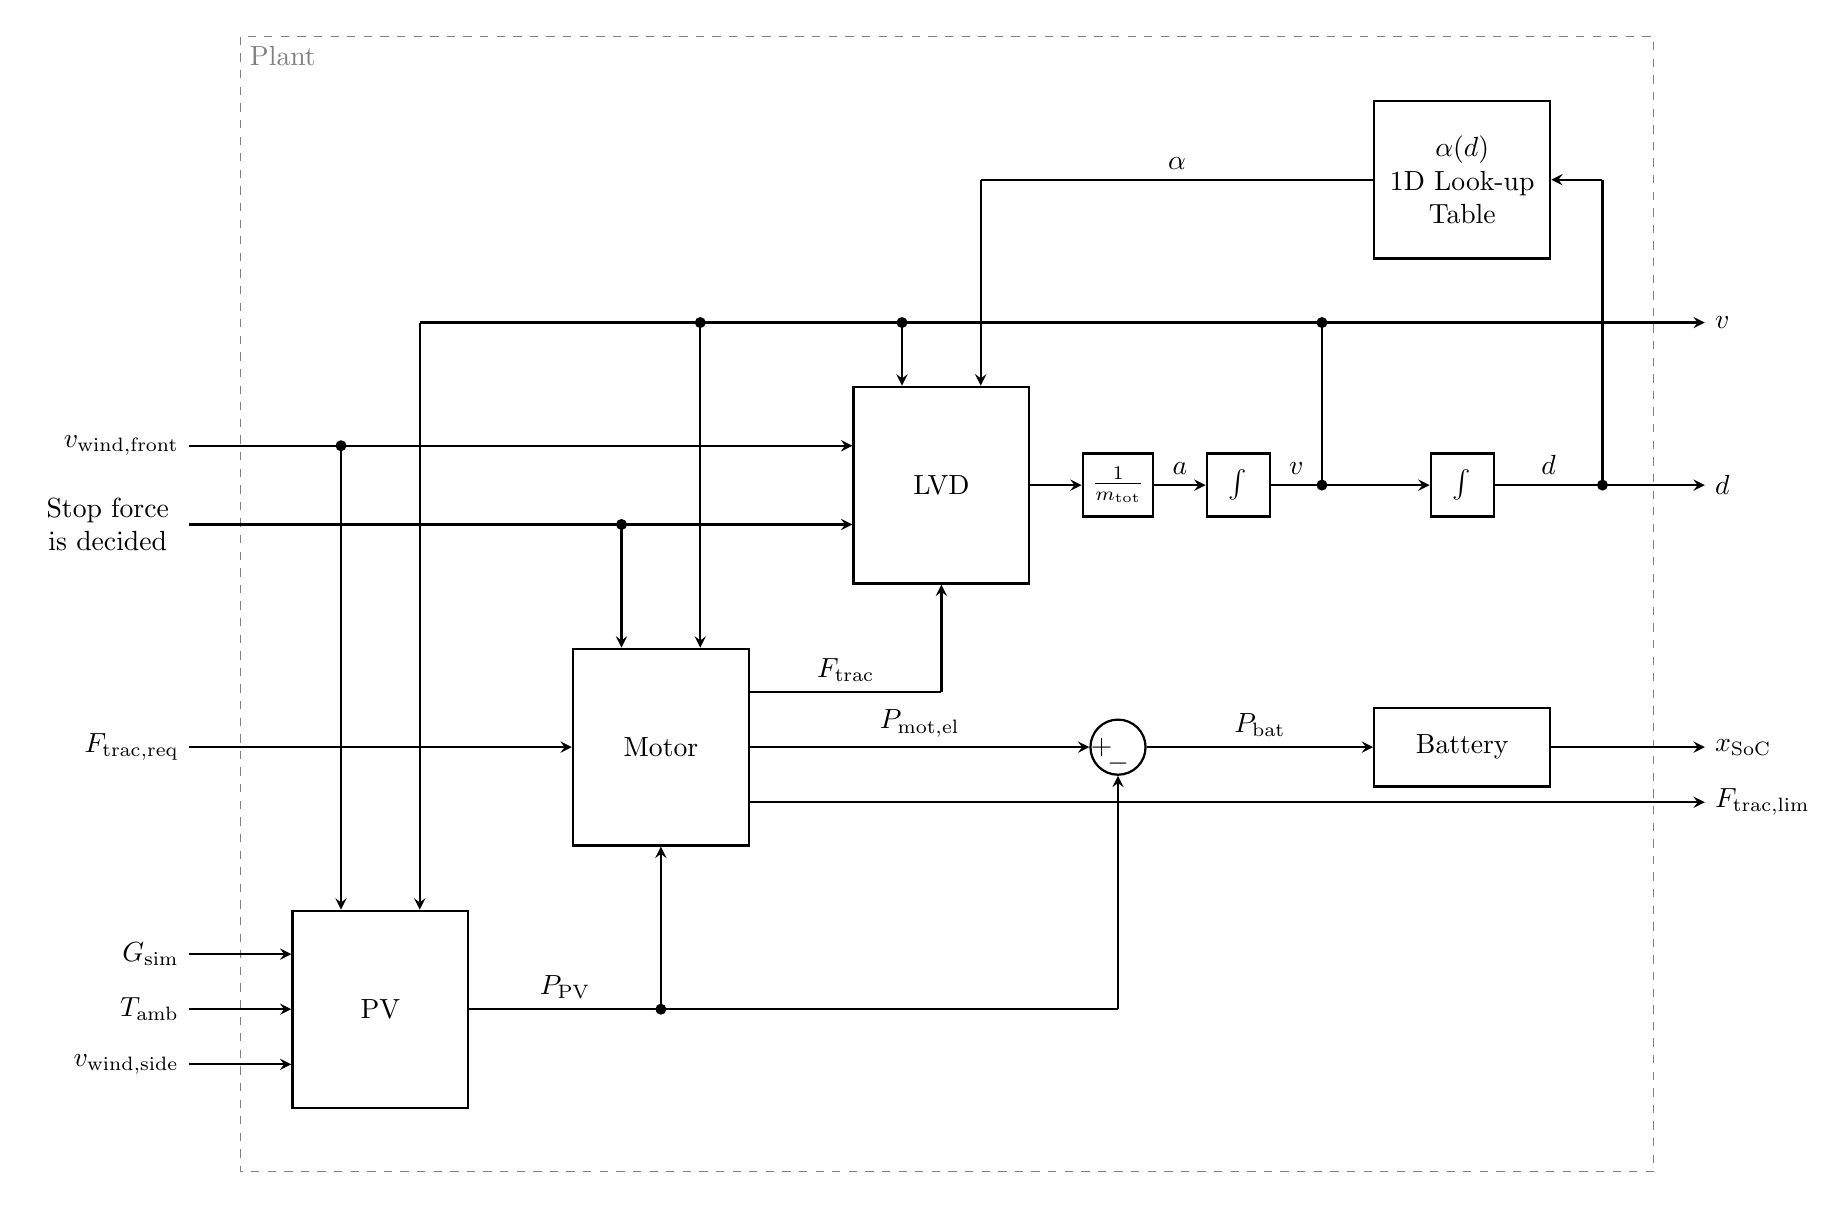
\begin{tikzpicture}
	% Definition
	%for three arrows
	\def\up{0.7}
	\def\down{-\up}
	\def\right{0.7}
	\def\left{-\right}
	%for two arrows
	\def\UP{0.5}
	\def\DOWN{-\UP}
	\def\RIGHT{0.5}
	\def\LEFT{-\RIGHT}
	%radius
	\def\radius{0.07}
	
	% Blocks
	\matrix[column sep=0.65cm, row sep=0.8cm]{
		%first row
		& \coordinate (c12); & & & &  & & & & &  & & & &
		\\
		%second row
		& & & & &  & \coordinate (c27); & & & &  \node[midBlock] (inclination) {$\alpha(d)$ \\ 1D Look-up Table}; & \coordinate (c212); & & &
		\\
		%third row
		& & \coordinate (c33); & & \coordinate (c35); &  & \coordinate (c37); & & & \coordinate (c310); &  & & & \coordinate (c314); &
		\\
		%fourth row
		\coordinate (c41); & & \coordinate (c43); & & \coordinate (c45); &  & \node[bigBlock] (lvd) {LVD}; & \node[smallBlock] (mass) {$\frac{1}{m_\mathrm{tot}}$}; & \node[smallBlock] (intAcc) {$\int$}; & \coordinate (c410); &  \node[smallBlock] (intVel) {$\int$}; & \coordinate (c412); & & \coordinate (c414); &
		\\
		%fifth row
		\coordinate (c51); & & & & \node[bigBlock] (motor) {Motor}; &  & \coordinate (c57); & \node[sum] (sum) {}; & & &  \node[midBlock, minimum height=1cm] (battery) {Battery}; & & & \coordinate (c514); &
		\\
		%sixth row
		\coordinate (c61); & & \node[bigBlock] (PV) {PV}; & & \coordinate (c65); &  & & \coordinate (c68); & & &  & & & &
		\\
		%seventh row
		& & & & &  & & & & &  & & \coordinate (c713); & &
		\\
	};
	
	% Container
	\draw[container] (c12) rectangle (c713);
	\node[gray, anchor=north west] at (c12.north west) {Plant};
	
	% Arrows;
	%to second row
	\draw[arrow] (c212) -- (inclination);
	\draw[line] (c412) -- (c212);
	\draw[line] (inclination) -- ([xshift=\RIGHT cm]c27) node[midway, above] {$\alpha$};
	%to third row
	\draw[arrow] ([xshift=\RIGHT cm]c33) -- (c314) node[textOutput] {$v$};
	\draw[line] (c410) -- (c310);
	\draw[arrow] ([xshift=\RIGHT cm]c27) -- ([xshift=\RIGHT cm]lvd.north);
	%to fourth row
	\draw[arrow] (c412) -- (c414) node[textOutput] {$d$};
	\draw[line] (intVel) -- (c412) node[midway, above] {$d$};
	\draw[arrow] ([yshift=\DOWN cm]c41) node[textInput, text width=1.8cm, text centered] {Stop force is decided} -- ([yshift=\DOWN cm]lvd.west);
	\draw[arrow] ([yshift=\UP cm]c41) node[textInput] {$v_\mathrm{wind,front}$} -- ([yshift=\UP cm]lvd.west);
	\draw[arrow] ([xshift=\LEFT cm]c37) -- ([xshift=\LEFT cm]lvd.north);
	\draw[arrow] (lvd) -- (mass);
	\draw[arrow] (mass) -- (intAcc) node[midway, above] {$a$};
	\draw[line] (intAcc) -- (c410) node[midway, above] {$v$};
	\draw[arrow] (c410) -- (intVel);
	\draw[arrow] ([yshift=\up cm]c57) -- (lvd);
	%to fifth row
	\draw[arrow] (battery) -- (c514) node[textOutput] {$x_\mathrm{SoC}$};
	\draw[arrow] (motor) -- (sum) node[midway, above] {$P_\mathrm{mot,el}$};
	\draw[arrow] (sum) -- (battery) node[midway, above] {$P_\mathrm{bat}$};
	\draw[arrow] ([xshift=\RIGHT cm]c35) -- ([xshift=\RIGHT cm]motor.north);
	\draw[arrow] (c68) -- (sum);
	\draw[line] (PV) -- (c65) node[midway, above] {$P_\mathrm{PV}$};
	\draw[arrow] (c65) -- (motor);
	\draw[arrow] (c51) node[textInput] {$F_\mathrm{trac,req}$} -- (motor.west);
	\draw[arrow] ([xshift=\LEFT cm, yshift=\DOWN cm]c45) -- ([xshift=\LEFT cm]motor.north);
	\draw[arrow] ([yshift=\down cm]motor.east) -- ([yshift=\down cm]c514) node[textOutput] {$F_\mathrm{trac,lim}$};
	\draw[line] ([yshift=\up cm]motor.east) -- ([yshift=\up cm]c57) node[midway, above] {$F_\mathrm{trac}$};
	%to sixth row
	\draw[arrow] (c61) node[textInput] {$T_\mathrm{amb}$} -- (PV);
	\draw[arrow] ([xshift=\RIGHT cm]c33) -- ([xshift=\RIGHT cm]PV.north);
	\draw[line] (PV) -- (c68);
	\draw[arrow] ([yshift=\up cm]c61) node[textInput] {$G_\mathrm{sim}$} -- ([yshift=\up cm]PV.west);
	\draw[arrow] ([yshift=\down cm]c61) node[textInput] {$v_\mathrm{wind,side}$} -- ([yshift=\down cm]PV.west);
	\draw[arrow] ([yshift=\UP cm, xshift=\LEFT cm]c43) -- ([xshift=\LEFT cm]PV.north);
	
	% Dots
	\fill [black] (c310) circle (\radius cm);
	\fill [black] ([xshift=\RIGHT cm]c35) circle (\radius cm);
	\fill [black] ([xshift=\LEFT cm]c37) circle (\radius cm);
	
	\fill [black] (c410) circle (\radius cm);
	\fill [black] (c412) circle (\radius cm);
	\fill [black] ([xshift=\LEFT cm, yshift=\DOWN cm]c45) circle (\radius cm);
	\fill [black] ([xshift=\LEFT cm, yshift=\UP cm]c43) circle (\radius cm);
	
	\fill [black] (c65) circle (\radius cm);
	
	%sum
	\path pic at (sum) {sum block={}{-}{+}{}};
	
\end{tikzpicture}
	\caption{Block diagram representation for the Plant.}
	\label{fig:simPlant}
\end{sidewaysfigure}
Here, six inputs are received, whereas four outputs are generated, as listed in~\cref{tab:simInOutPlant}.
\begin{table}[htbp]
	\centering
	\caption{Input/Output signals for the Plant.}
	\label{tab:simInOutPlant}
	
	\begin{tabular}{c l l l l}
		\toprule
		& Block & Signal & Symbol & Type \\ 
		\midrule
		\multirow{6}{*}{Input from}
		& Driver & Requested traction force & $F_\mathrm{trac,req}$ & Float \\
		& Driver & Stop force is decided & -- & Binary \\
		& Weather & Global irradiance & $G_\mathrm{sim}$ & Float \\
		& Weather & Ambient temperature & $T_\mathrm{amb}$ & Float \\
		& Weather & Side wind speed & $v_\mathrm{wind,side}$ & Float \\
		& Weather & Frontal wind speed & $v_\mathrm{wind,front}$ & Float \\

		\midrule
		\multirow{4}{*}{Output to}
		& Weather and Driver & Car velocity & $v$ & Float \\
		& Weather and Driver & Driven distance & $d$ & Float \\
		& Driver & SoC & $x_\mathrm{SoC}$ & Float \\
		& Driver & Traction force bounds & $F_\mathrm{trac,lim}$ & Float \\
		\bottomrule
	\end{tabular}
\end{table}

The other important building blocks of the Plant shown in the figure are the following:
\begin{itemize}
	\item A one dimensional \texttt{Look-up Table} that interpolates the distance traveled from the starting line to obtain the route inclination;
	\item A \texttt{Gain} block that receives the inertial force $m_\mathrm{tot} \frac{d}{dt} v(t)$ from LVD and outputs the car acceleration;
	\item Two \texttt{Integrators} in series to generate the actual car velocity and position. Both initial conditions are set to zero, representing a standing start of the race; and
	\item A \texttt{Sum} block that guarantees that the power balance equation of~\cref{sec:modelPowerBalance} is fulfilled.
\end{itemize}


\subsection{Longitudinal Vehicle Dynamics}
\label{sec:simLVD}
The \texttt{Subsystem} for the LVD includes the implementation of the equations described in~\cref{sec:modelLVD}. The road inclination is taken into account, and the forces of rolling resistance $F_\mathrm{roll}$ and gravity $F_\mathrm{grav}$ are not approximated. For this reason, five inputs are necessary, while there is only one output, as listed in~\cref{tab:simInOutLVD}.
\begin{table}[htbp]
	\centering
	\caption{Input/Output signals for the LVD.}
	\label{tab:simInOutLVD}
	
	\begin{tabular}{c l l l l}
		\toprule
		& Block & Signal & Symbol & Type \\ 
		\midrule
		\multirow{5}{*}{Input from}
		& -- & Road inclination & $\alpha$ & Float \\
		& Weather & Car velocity & $v$ & Float \\
		& Weather & Frontal wind speed & $v_\mathrm{wind,front}$ & Float \\
		& Driver & Stop force is decided & -- & Binary \\
		& Motor & Traction force & $F_\mathrm{trac}$ & Float \\
		\midrule
		\multirow{1}{*}{Output to}
		& Internal & Inertial force & $m_\mathrm{tot} \frac{d}{dt} v(t)$ & Float \\
		\bottomrule
	\end{tabular}
\end{table}

The LVD implementation differs from the modeling equations by an additional friction force created with a \texttt{Coulomb \& Viscous Friction} block. It is turned on with the boolean signal \enquote{Stop force is decided} from the Driver, which at the same time deactivates the other friction forces. This corresponds to the effect of activating a hand brake system, necessary to keep the velocity at a constant zero during the control and overnight stops without consuming electrical power.


\subsection{Electric Motor}
\label{sec:simMotor}
This \texttt{Subsystem} is divided into two parts: the first one calculates the bounds used in the Controllers \texttt{Subsystem} of~\cref{sec:simDriver}, while the second one contains the model equations.

Four inputs are received and three outputs generated, as listed in~\cref{tab:simInOutMotor}.
\begin{table}[htbp]
	\centering
	\caption{Input/Output signals for the Motor.}
	\label{tab:simInOutMotor}
	
	\begin{tabular}{c l l l l}
		\toprule
		& Block & Signal & Symbol & Type \\ 
		\midrule
		\multirow{4}{*}{Input from}
		& -- & Car velocity & $v$ & Float \\
		& Driver & Stop force is decided & -- & Binary \\
		& Driver & Requested traction force & $F_\mathrm{trac,req}$ & Float \\
		& PV & PV power & $P_\mathrm{PV}$ & Float \\
		\midrule
		\multirow{3}{*}{Output to}
		& LVD & Traction force & $F_\mathrm{trac}$ & Float \\
		& Sum & Electric motor power & $P_\mathrm{mot,el}$ & Float \\
		& Driver & Traction force bounds & $F_\mathrm{trac,lim}$ & Float \\
		\bottomrule
	\end{tabular}
\end{table}


\paragraph{Bounds Calculator}
This \texttt{MATLAB Function} contains the codes that generates the maximal and minimal mechanical torque that can be provided by the electric motor. These values are determined by considering all the limits of the motor described in~\cref{sec:modelMotor} and the battery limits from~\cref{sec:modelBattery}. The integration of these limits requires rewriting~\cref{eq:powerBalance} for the electric motor power, which leads to the following upper bounds:
\begin{align}
	P_\mathrm{mot,el} &\leq P_\mathrm{bat,max} + P_\mathrm{PV}, \\
	P_\mathrm{mot,el} &\leq I_\mathrm{bat,max} \cdot \left( U_\mathrm{bat,oc} - R_\mathrm{bat} \cdot I_\mathrm{bat,max} \right) + P_\mathrm{PV}, \\
	P_\mathrm{mot,el} &\leq \frac{U_\mathrm{bat,oc}^2}{4 \cdot R_\mathrm{bat}} + P_\mathrm{PV}.
\end{align}
While for the lower limits holds:
\begin{align}
	P_\mathrm{mot,el} &\geq P_\mathrm{bat,min} + P_\mathrm{PV}, \\
	P_\mathrm{mot,el} &\geq I_\mathrm{bat,min} \cdot \left( U_\mathrm{bat,oc} - R_\mathrm{bat} \cdot I_\mathrm{bat,min} \right) + P_\mathrm{PV}.
\end{align}
Furthermore, numerical problems arise when dividing with a velocity approaching zero to convert power to forces or torques. For this reason, \texttt{Saturation} blocks and explicit division with a small number is implemented. The torque signals are converted to forces and sent to the Driver block as $F_\mathrm{trac,lim}$.

\paragraph{Motor}
The modeling equations derived in~\cref{sec:modelMotor} are written in this \texttt{MATLAB Function}, including the limits and the torque bounds calculated in the Bounds Calculator.

In case of strong braking, not all the power can be recuperated in the battery. Therefore, a dissipative braking force is also calculated here.


\subsection{PV Module}
\label{sec:simPV}
In this subsystem, the model derived in~\cref{sec:modelPV} is included in a \texttt{MATLAB Function}. Five inputs are received, while only one output is generated, as listed in~\cref{tab:simInOutPV}.
\begin{table}[htbp]
	\centering
	\caption{Input/Output signals for the PV.}
	\label{tab:simInOutPV}
	
	\begin{tabular}{c l l l l}
		\toprule
		& Block & Signal & Symbol & Type \\ 
		\midrule
		\multirow{5}{*}{Input from}
		& -- & Car velocity & $v$ & Float \\
		& Weather & Frontal wind speed & $v_\mathrm{wind,front}$ & Float \\
		& Weather & Global irradiance & $G_\mathrm{sim}$ & Float \\
		& Weather & Ambient temperature & $T_\mathrm{amb}$ & Float \\
		& Weather & Side wind speed & $v_\mathrm{wind,side}$ & Float \\
		\midrule
		\multirow{1}{*}{Output to}
		& Motor and sum & PV power & $P_\mathrm{PV}$ & Float \\
		\bottomrule
	\end{tabular}
\end{table}

\subsection{Battery Pack}
\label{sec:simBattery}
The model of the battery pack described in~\cref{sec:modelBattery} is implemented in Simulink using a series of basic blocks. The model begins with a \texttt{MATLAB function} block, followed by an \texttt{Integrator} block to calculate the actual charge, a \texttt{Gain} block to determine the SoC, and a \texttt{Saturation} block to prevent the SoC from exceeding the limit of $\unit[100]{\%}$. Any additional power supplied to the battery after this limit is reached, is assumed to be converted into heat.

As previously mentioned, the battery limits are not included in this subsystem, but rather in the electric motor block of~\cref{sec:simMotor}. This is necessary to ensure that the causality of the Simulink simulation is preserved.

Only one input is received, and one output is generated as listed in~\cref{tab:simInOutBattery}.
\begin{table}[htbp]
	\centering
	\caption{Input/Output signals for the Battery.}
	\label{tab:simInOutBattery}
	
	\begin{tabular}{c l l l l}
		\toprule
		& Block & Signal & Symbol & Type \\ 
		\midrule
		\multirow{1}{*}{Input from}
		& Sum & Battery power & $P_\mathrm{bat}$ & Float \\
		\midrule
		\multirow{1}{*}{Output to}
		& Controllers & SoC & $x_\mathrm{SoC}$ & Float \\
		\bottomrule
	\end{tabular}
\end{table}

\newpage
\section{Weather}
\label{sec:simWeather}
The analysis of the weather data of~\cref{sec:modelingWeatherData} and their conversion in seconds allow the implementation of this component with the mere usage of \texttt{Look-up Tables}: two dimensional tables are needed for the ambient temperature and wind speeds, while a one dimensional one is used for the global irradiance.~\Cref{fig:simWeather} shows the block diagram representation of this \texttt{Subsystem}, where the interpolations take place.

Two inputs are received, whereas four outputs are generated as listed in~\cref{tab:simInOutWeather}.
\begin{table}[htbp]
	\centering
	\caption{Input/Output signals for the Weather.}
	\label{tab:simInOutWeather}
	
	\begin{tabular}{c l l l l}
		\toprule
		& Block & Signal & Symbol & Type \\ 
		\midrule
		\multirow{2}{*}{Input from}
		& Simulink & Absolute time & $t_\mathrm{sim}$ & Float \\
		& Plant & Driven distance & $d$ & Float \\
		\midrule
		\multirow{4}{*}{Output to}
		& Plant & Global irradiance & $G_\mathrm{sim}$ & Float \\
		& Plant & Ambient temperature & $T_\mathrm{amb}$ & Float \\
		& Plant & Side wind speed & $v_\mathrm{wind,side}$ & Float \\
		& Plant & Frontal wind speed & $v_\mathrm{wind,front}$ & Float \\
		\bottomrule
	\end{tabular}
\end{table}

\begin{figure}[htbp]
	\centering
	% Styles
\tikzstyle{block} = [rectangle, thick, minimum width=2.5cm, minimum height=1.5cm,text centered, text width=3cm, draw=black, fill=white]
\tikzstyle{arrow} = [thick, ->, >=stealth]
\tikzstyle{textOutput} = [black,right]
\tikzstyle{textInput} = [black,left]
\tikzstyle{container} = [gray,dashed]

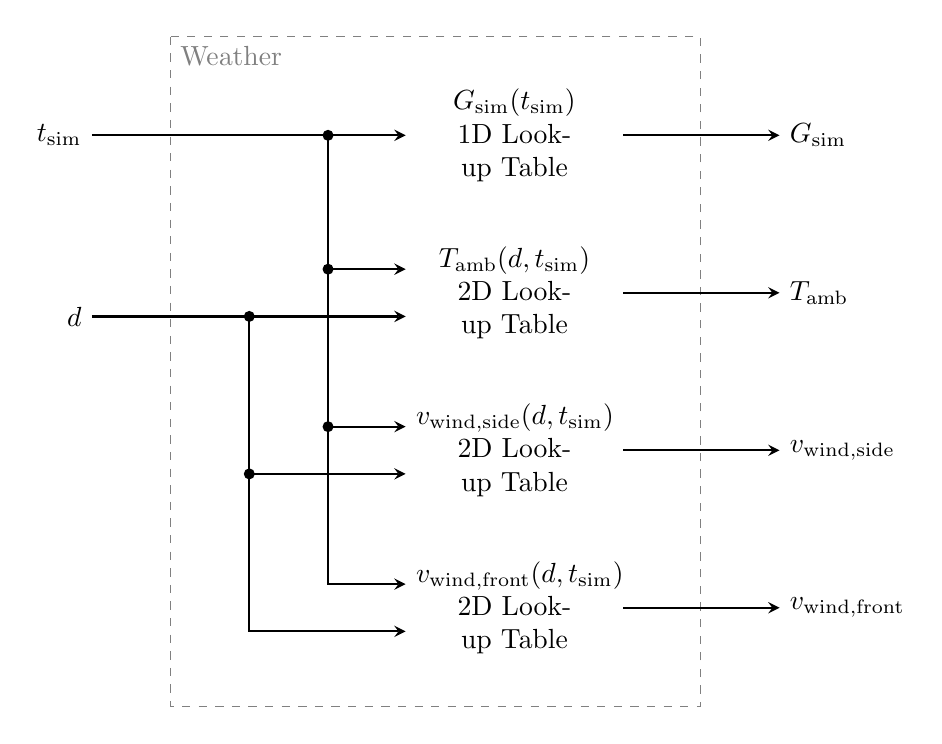
\begin{tikzpicture}
	% Definition
	\def\up{0.3}
	\def\down{-\up}
	\def\radius{0.07}
	
	% Blocks
	\matrix[column sep=1cm, row sep=0.5cm]{
		%first row
		& \coordinate (c12); & & & & & &
		\\
		%second row
		\coordinate (c21); & & & \coordinate (c24); & \node[block] (G) {$G_\mathrm{sim}(t_\mathrm{sim})$ \\ 1D Look-up Table}; & & \coordinate (c27); &
		\\
		%third row
		\coordinate (c31); & & \coordinate (c33); & \coordinate (c34); & \node[block] (T) {$T_\mathrm{amb}(d,t_\mathrm{sim})$ \\ 2D Look-up Table}; & & \coordinate (c37); &
		\\
		%fourth row
		& & \coordinate (c43); & \coordinate (c44); & \node[block] (vs) {$v_\mathrm{wind,side}(d,t_\mathrm{sim})$ \\ 2D Look-up Table}; & & \coordinate (c47); &
		\\
		%fifth row
		& & \coordinate (c53); & \coordinate (c54); & \node[block] (vf) {$v_\mathrm{wind,front}(d,t_\mathrm{sim})$ \\ 2D Look-up Table}; & & \coordinate (c57); &
		\\
		%sixth row
		& & & & & \coordinate (c66); & &
		\\
	};
	
	% Container
	\draw[container] (c12) rectangle (c66);
	\node[gray, anchor=north west] at (c12.north west) {Weather};
	
	% Arrows
	\draw[arrow] (c21) node[textInput] {$t_\mathrm{sim}$} -- (G);
	\draw[arrow] (G) -- (c27) node[textOutput] {$G_\mathrm{sim}$};
	
	\draw[arrow] ([yshift=\down cm]c31) node[textInput] {$d$} -- ([yshift=\down cm]T.west);
	\draw[arrow] (T) -- (c37) node[textOutput] {$T_\mathrm{amb}$};
	\draw[arrow] ([yshift=\up cm]c34) -- ([yshift=\up cm]T.west);
	
	\draw[arrow] (vs) -- (c47) node[textOutput] {$v_\mathrm{wind,side}$};
	\draw[arrow] ([yshift=\up cm]c44) -- ([yshift=\up cm]vs.west);
	\draw[arrow] ([yshift=\down cm]c43) -- ([yshift=\down cm]vs.west);
	
	\draw[arrow] (vf) -- (c57) node[textOutput] {$v_\mathrm{wind,front}$};
	\draw[arrow] ([yshift=\down cm]c33) -- ([yshift=\down cm]c53) -- ([yshift=\down cm]vf.west);
	\draw[arrow] (c24) -- ([yshift=\up cm]c54) -- ([yshift=\up cm]vf.west);
	
	% Dots
	\fill [black] (c24) circle (\radius cm);
	
	\fill [black] ([yshift=\up cm]c34) circle (\radius cm);
	\fill [black] ([yshift=\down cm]c33) circle (\radius cm);
	
	\fill [black] ([yshift=\up cm]c44) circle (\radius cm);
	\fill [black] ([yshift=\down cm]c43) circle (\radius cm);

	
\end{tikzpicture}
	\caption{Block diagram representation for the Weather.}
	\label{fig:simWeather}
\end{figure}

Alternatives to \texttt{Look-up Tables} are discarded because of the their slower computational performance with respect to these Simulink built-in blocks. Direct interpolation in Matlab and the usage of \texttt{Gridded Interpolant} were tested.

\newpage
\section{Driver}
\label{sec:simDriver}
The last of the three main components is the Driver, which is composed of a Decision Maker, a Controllers \texttt{Subsystem}, and three one dimensional \texttt{Look-up Tables}, as illustrated in~\cref{fig:simDriver}. The first table outputs the speed limit $v_\mathrm{max}$ at the current car position on the route, the second one provides the number of the current race day (day one is the 20. October), and the third outputs \enquote{true} when driving during the day is possible, namely from 10:00 to 17:00 on day one and from 08:00 to 17:00 for the rest of the race.
\begin{sidewaysfigure}[htbp]
	\centering
	% Styles
\tikzset{
	lookBlock/.style = {rectangle, thick, minimum width=2.5cm, minimum height=1.5cm,text centered, text width=3cm, draw=black, fill=white},
	block/.style = {rectangle, thick, minimum width=2.5cm, minimum height=1.5cm,text centered, text width=2.5cm, draw=none, fill=white},
	arrow/.style= {thick, black, ->, >=stealth},
	line/.style= {thick, black},
	textOutput/.style = {black,right},
	textInput/.style = {black,left},
	container/.style = {gray,dashed}
}

\begin{tikzpicture}
	% Definition
	%for three arrows
	\def\right{0.8}
	\def\left{-\right}
	%for two arrows
	\def\UP{0.55}
	\def\DOWN{-\UP}
	%radius
	\def\radius{0.07}
	
	% Blocks
	\matrix[column sep=1.3cm, row sep=0.7cm]{
		%first row
		& \coordinate (c12); & & & &  & & & & &
		\\
		%second row
		\coordinate (c21); & & & & &  & & \node[block] (C1) {}; & & &
		\\
		%third row
		\coordinate (c31); & & \coordinate (c33); & & &  & \coordinate (c37); & \node[block] (C2) {}; & & &
		\\
		%fourth row
		\coordinate (c41); & & & \coordinate (c44); & &  \coordinate (c46); & \coordinate (c47); & \node[block] (C3) {}; & & \coordinate (c410); &
		\\
		%fifth row
		& & & \coordinate (c54); & \node[lookBlock] (MS) {$v_\mathrm{max}(d)$ \\ 1D Look-up Table}; &  \coordinate (c56); & \node[block] (D1) {}; & \node[block] (C4) {}; & & &
		\\
		%sixth row
		& & \coordinate (c63); & & \node[lookBlock] (DN) {Day number$(t_\mathrm{sim})$ \\ 1D Look-up Table}; &  & \node[block] (D2) {}; & \node[block] (C5) {}; & & &
		\\
		%seventh row
		& & \coordinate (c73); & & \node[lookBlock] (Driving) {Driving is needed$(t_\mathrm{sim})$ \\ 1D Look-up Table}; &  & \node[block] (D3) {}; & \node[block] (C6) {}; & & &
		\\
		%eigth row
		& & & & &  & \coordinate (c87); & & & \coordinate (c810); &
		\\
		%ninth row
		& & & & &  & & & \coordinate (c99); & &
		\\
	};
	
	% Container
	\draw[container] (c12) rectangle (c99);
	\node[gray, anchor=north west] at (c12.north west) {Driver};
	
	% Arrows
	%to second
	\draw[arrow] ([yshift=\UP cm]c21) node[textInput] {$x_\mathrm{SoC}$} -- ([yshift=\UP cm]C1.west);
	\draw[arrow] ([yshift=\DOWN cm]c21) node[textInput] {$F_\mathrm{trac,lim}$} -- ([yshift=\DOWN cm]C1.west);
	%to third
	\draw[arrow] ([yshift=\UP cm]c31) node[textInput] {$v$} -- ([yshift=\UP cm]C2.west);
	\draw[arrow] ([yshift=\DOWN cm]c31) node[textInput] {$t_\mathrm{sim}$} -- ([yshift=\DOWN cm]C2.west);
	%to fourth
	\draw[arrow] ([yshift=\DOWN cm]C3.east) -- ([yshift=\DOWN cm]c410) node[textOutput] {$F_\mathrm{trac,req}$};
	\draw[arrow] ([yshift=\UP cm]c41) node[textInput] {$d$} -- ([yshift=\UP cm]C3.west);
	\draw[arrow] ([yshift=\DOWN cm]c46) -- ([yshift=\DOWN cm]C3.west);
	%to fifth
	\draw[line] ([yshift=\UP cm]c44) -- (c54);
	\draw[arrow] (c54) -- (MS);
	\draw[line] (MS) -- (c56) node[midway, above] {$v_\mathrm{max}$};
	\draw[arrow] (c56) -- (D1);
	\draw[line] ([yshift=\DOWN cm]c46) -- (c56);
	\draw[arrow] (D1) -- (C4) node[midway, above, text width=1.2cm, text centered] {Acc is dec};
	\draw[arrow] ([yshift=\UP cm, xshift=\left cm]c47) -- ([xshift=\left cm]D1.north);
	\draw[arrow] ([yshift=\DOWN cm]c37) -- (D1);
	\draw[arrow] ([yshift=\UP cm, xshift=\right cm]c37) -- ([xshift=\right cm]D1.north);
	%to sixth
	\draw[arrow] (c63) -- (DN);
	\draw[arrow] (DN) -- (D2);
	\draw[arrow] (D2) -- (C5) node[midway, above, text width=1.2cm, text centered] {Dec is dec};
	%to seventh
	\draw[line] ([yshift=\DOWN cm]c33) -- (c73);
	\draw[arrow] (c73) -- (Driving);
	\draw[arrow] (Driving) -- (D3);
	\draw[arrow] (D3) -- (C6) node[midway, above, text width=1.2cm, text centered] {Cruise is dec};
	%to eigth
	\draw[line] (D3) -- (c87);
	\draw[arrow] (c87) -- (c810) node[textOutput, text width=1.8cm, text centered] {Stop force is decided};
	
	% Dots
	\fill [black] ([yshift=\DOWN cm]c33) circle (\radius cm);
	\fill [black] ([yshift=\DOWN cm]c37) circle (\radius cm);
	\fill [black] ([yshift=\UP cm, xshift=\right cm]c37) circle (\radius cm);
	
	\fill [black] ([yshift=\UP cm]c44) circle (\radius cm);
	\fill [black] ([yshift=\UP cm, xshift=\left cm]c47) circle (\radius cm);
	
	\fill [black] (c56) circle (\radius cm);
	
	\fill [black] (c63) circle (\radius cm);
	
	%Fit
	\node [inner sep=-0.5\pgflinewidth,fit=(D1)(D2)(D3), draw] {Decision \\ Maker};
	\node [inner sep=-0.5\pgflinewidth,fit=(C1)(C2)(C3)(C4)(C5)(C6), draw] {Controllers};
	
	
\end{tikzpicture}
	\caption{Block diagram representation of the Driver.}
	\label{fig:simDriver}
\end{sidewaysfigure}

Five inputs are received, whereas two outputs are generated, as listed in~\cref{tab:simInOutDriver}.
\begin{table}[htbp]
	\centering
	\caption{Input/Output signals for the Driver.}
	\label{tab:simInOutDriver}
	
	\begin{tabular}{c l l l l}
		\toprule
		& Block & Signal & Symbol & Type \\ 
		\midrule
		\multirow{5}{*}{Input from}
		& Plant & SoC & $x_\mathrm{SoC}$ & Float \\
		& Plant & Traction force bounds & $F_\mathrm{trac,lim}$ & Float \\
		& Plant & Car velocity & $v$ & Float \\
		& Simulink & Absolute time & $t_\mathrm{sim}$ & Float \\
		& Plant & Driven distance & $d$ & Float \\
		\midrule
		\multirow{2}{*}{Output to}
		& Plant & Requested traction force & $F_\mathrm{trac,req}$ & Float \\
		& Plant & Stop force is decided & -- & Binary \\
		\bottomrule
	\end{tabular}
\end{table}


\subsection{Decision Maker}
This \texttt{MATLAB Function} represents the brain of the Driver, where velocity and position of the car as well as route information are processed to decide what action has to be perform by the actuators in the Controllers or in the Plant. Additionally, some variables are saved in the Simulink memory data storage, therefore simulating some sort of memory. The six signals received and the four generated binary signals are listed in~\cref{tab:simInOutDecisionMaker}.
\begin{table}[htbp]
	\centering
	\caption{Input/Output signals for the Decision Maker.}
	\label{tab:simInOutDecisionMaker}
	
	\begin{tabular}{c l l l l}
		\toprule
		& Block & Signal & Symbol & Type \\ 
		\midrule
		\multirow{6}{*}{Input from}
		& Simulink & Absolute time & $t_\mathrm{sim}$ & Float \\
		& Plant & Driven distance & $d$ & Float \\
		& Plant & Car velocity & $v$ & Float \\
		& -- & Maximal speed & $v_\mathrm{max}$ & Float \\
		& -- & Day number & -- & Integer \\
		& -- & Driving is needed & -- & Binary \\
		\midrule
		\multirow{4}{*}{Output to}
		& Controllers & Acceleration is decided & Acc is dec & Binary \\
		& Controllers & Deceleration is decided & Dec is dec & Binary \\
		& Controllers & Cruise is decided & Cruise is dec & Binary \\
		& Plant & Stop force is decided & -- & Binary \\
		\bottomrule
	\end{tabular}
\end{table}

The decision process is written with logical statements, where only one output signal of this subsystem can be \enquote{true} at every time. First, the equation of motion helps finding when a control stop is approaching or the driving day has come to an end:
\begin{equation}
\begin{cases}
	d(t) = d_0 + v_0 \cdot t + \frac{1}{2} \cdot a \cdot t^2 \\
	v(t) = v_0 + a \cdot t \\
	a(t) = f(t)
\end{cases} \label{eq:simEqOfMotion}
\end{equation}
where $d_0$ is the current position or distance traveled from the starting line, $v_0$ is the current velocity, $t$ is the time, and $a$ is the acceleration.

In case of a control stop, it is necessary to check whether the distance traveled with constant deceleration $a_\mathrm{dec}$ from the current position $d_\mathrm{s}$ is greater or equal the distance to the next control stop $d_\mathrm{ns}$:
\begin{equation}
	d_\mathrm{s} \geq d_\mathrm{ns},
\end{equation}
where $d_\mathrm{s}$ is found using the equation of motion~\cref{eq:simEqOfMotion}:
\begin{equation}
	d_\mathrm{s} = d_0 - \frac{v_0^2}{2 \cdot a_\mathrm{dec}}.
\end{equation}

Similarly for the driving time stops, it is necessary to check whether the time to come to a stop $t_\mathrm{s}$ is greater or equal 16:59 in Simulink time $t_\mathrm{ns}$ (the overnight stops happen approximately one minute before 17:00):
\begin{equation}
	t_\mathrm{s} \geq t_\mathrm{ns},
\end{equation}
where $t_\mathrm{s}$ is also found using the equation of motion~\cref{eq:simEqOfMotion}:
\begin{equation}
	t_\mathrm{s} = t_0 + \frac{v_0}{a_\mathrm{dec}}.
\end{equation}

The variables \enquote{Day number} and \enquote{Driving is needed} are used to decide to accelerate at the beginning of a racing day. The acceleration after a control stop is decided once 30 minutes have passed. The Decision Maker is presented in~\cref{fig:simStateMachine} as a finite state machine.
\begin{figure}[htbp]
	\centering
	\begin{tikzpicture}[node distance=5cm, >=stealth',
	every state/.style={circle, minimum size=3cm, thick, draw=black, fill=gray!20!white}]
	\node[state, initial, text width=2 cm, align=center] (acc) {Acceleration is decided};
	\node[state] (cruise) [right of=acc, text width=2 cm, align=center] {Cruise is decided};
	\node[state] (dec) [below of=cruise, text width=2 cm, align=center] {Deceleration is decided};
	\node[state] (stop) [left of=dec, text width=2 cm, align=center] {Stop force is decided};
	\path[->] (acc) edge [loop above] node {$\textbf{if } v < \min(v_\mathrm{max}, v_\mathrm{ref})$} (acc);
	\path[->] (acc) edge [bend left] node[above] {\textbf{else}} (cruise);
	\path[->] (cruise) edge [loop right] node {\textbf{else}} (cruise);
	\path[->] (cruise) edge [bend left] node[right] {$\textbf{if } d_\mathrm{s} \geq d_\mathrm{ns} \textbf{ or } t_\mathrm{s} \geq t_\mathrm{ns}$} (dec);
	\path[->] (dec) edge [loop right] node {$\textbf{if } v > 0$} (dec);
	\path[->] (dec) edge [bend left] node[below] {\textbf{else}} (stop);
	\path[->] (stop) edge [loop left] node {\textbf{else}} (stop);
	\path[->] (stop) edge [bend left] node[left, text width=4.5 cm] {\textbf{if} \enquote{Racing day is started} \\ \textbf{or} \enquote{Control stop is over}} (acc);
\end{tikzpicture}
	\caption{Finite state machine of the Decision Maker with the four control modes.}
	\label{fig:simStateMachine}
\end{figure}
%\begin{algorithm}
%	\caption{Decision Maker pseudocode.}
%	\label{alg:decisionMaker}
%	\begin{algorithmic}
%	\Input{Training sentences $S_{i}$}
%	\Output{Sentence instances with cost-vectors for training $S_{i,c_i}$}
	\State Check if a control stop is approaching: $d_\mathrm{s} \geq d_\mathrm{ns}$
	\State Check if the end of the day is near: $t_\mathrm{s} \geq t_\mathrm{ns}$
	\State Check if the racing day is started
	\If{\enquote{Overnight stop is needed}}  \Comment{Deceleration}
	\If{$v > 0$}
	\State \enquote{Deceleration is decided} $\gets$ "true"
	\Else
	\State \enquote{Stop force is decided} $\gets$ "true"
	\EndIf
	\ElsIf{\enquote{Control stop is needed}}
	\If{$v > 0$}
	\State \enquote{Deceleration is decided} $\gets$ "true"
	\Else
	\State \enquote{Stop force is decided} $\gets$ "true"
	\If{30 minutes have passed}
	\State \enquote{Control stop is over} $\gets$ "true"
	\EndIf
	\EndIf
	\ElsIf{\enquote{Racing day is started}}  \Comment{Acceleration}
	\If{$v < 0.9 \cdot \min(v_\mathrm{max}, v_\mathrm{ref})$}
	\State \enquote{Acceleration is decided} $\gets$ "true"
	\Else
	\State \enquote{Cruise is decided} $\gets$ "true"
	\EndIf
	\ElsIf{\enquote{Control stop is over}}
	\If{$v < 0.9 \cdot \min(v_\mathrm{max}, v_\mathrm{ref})$}
	\State \enquote{Acceleration is decided} $\gets$ "true"
	\Else
	\State \enquote{Cruise is decided} $\gets$ "true"
	\EndIf
	\Else
	\State \enquote{Cruise is decided} $\gets$ "true"  \Comment{Cruise}
	\EndIf

\end{algorithmic}
%\end{algorithm}


\subsection{Controllers}
\label{sec:simDriverControllers}
In this \texttt{Subsystem}, human-like behavior is simulated using a combination of two PI controllers and one cascaded controller. The latter is primarily responsible for setting the cruising velocity, while the formers handle acceleration and deceleration.

In Simulink, the maximal step size is set to $\unit[0.2]{s}$ to prevent divergent behavior of the controllers. If the step size is set to a larger value, the controllers may become unstable.

Nine inputs are received and only one output is generated as listed in~\cref{tab:simInOutControllers}.
\begin{table}[htbp]
	\centering
	\caption{Input/Output signals for the Controllers.}
	\label{tab:simInOutControllers}
	
	\begin{tabular}{c l l l l}
		\toprule
		& Block & Signal & Symbol & Type \\ 
		\midrule
		\multirow{9}{*}{Input from}
		& Plant & SoC & $x_\mathrm{SoC}$ & Float \\
		& Plant & Traction force bounds & $F_\mathrm{trac,lim}$ & Float \\
		& Plant & Car velocity & $v$ & Float \\
		& Simulink & Absolute time & $t_\mathrm{sim}$ & Float \\
		& Plant & Driven distance & $d$ & Float \\
		& -- & Maximal speed & $v_\mathrm{max}$ & Float \\
		& Decision Maker & Acceleration is decided & Acc is dec & Binary \\
		& Decision Maker & Deceleration is decided & Dec is dec & Binary \\
		& Decision Maker & Cruise is decided & Cruise is dec & Binary \\
		\midrule
		\multirow{1}{*}{Output to}
		& Plant & Requested traction force & $F_\mathrm{trac,req}$ & Float \\
		\bottomrule
	\end{tabular}
\end{table}

\paragraph{Acceleration and Deceleration}
These two \texttt{Subsystems} are constructed in the same way, with the only exception of a positive or negative constant acceleration in the code, $a_\mathrm{acc}$ or $a_\mathrm{dec}$, respectively.

As soon as acceleration or deceleration is decided, time and car velocity values are stored in the memory. These parameters are used to generate the corresponding reference ramp velocity $v_\mathrm{ref}$ with constant slope. The difference between reference and actual velocity $v_\mathrm{ref} - v$ used as input to the \texttt{PID(s)} built-in block, where the traction force bounds ensure that the output requested traction force is limited and that the integral term does not saturate. For this purpose, the clamping anti-reset windup (ARW) is activated.

\paragraph{Cruise}
For the majority of the time, a more or less constant reference velocity $v_\mathrm{ref}$ has to be followed. Its value is estimated considering the current SoC value, as illustrated in~\cref{fig:simCascadedController}. This single input multiple output behavior is achieved with a cascaded controller, where the fast PI controller converts velocity in requested traction force, while the slow PI controller translates SoC values into velocity. In case a higher SoC than the reference is detected, the velocity is increased to consume the extra energy stored in the battery. The opposite is true for a lower SoC detection.
\begin{sidewaysfigure}[htbp]
	\centering
	% Styles
\tikzset{
	midBlock/.style = {rectangle, thick, minimum width=2cm, minimum height=2cm,text centered, text width=2cm, draw=black, fill=white},
	arrow/.style= {thick, black, ->, >=stealth},
	line/.style= {thick, black},
	textOutput/.style = {black,right},
	textInput/.style = {black,left},
	container/.style = {gray,dashed},
	sum/.style = {circle, minimum size=0.7cm, thick, draw=black, fill=white},
	%sum
	charge node/.style={inner sep=0pt},
	pics/sum block/.style n args={4}{
		code={
			\path node (n) [draw, circle, inner sep=0pt, minimum size=0.7cm] {}
			(n.north) +(0,-1.5mm) node [charge node] {$#1$}
			(n.south) +(0,1.5mm) node [charge node] {$#2$}
			(n.west) +(1.5mm,0) node [charge node] {$#3$}
			(n.east) +(-1.5mm,0) node [charge node] {$#4$}
			;
		}
	}
}
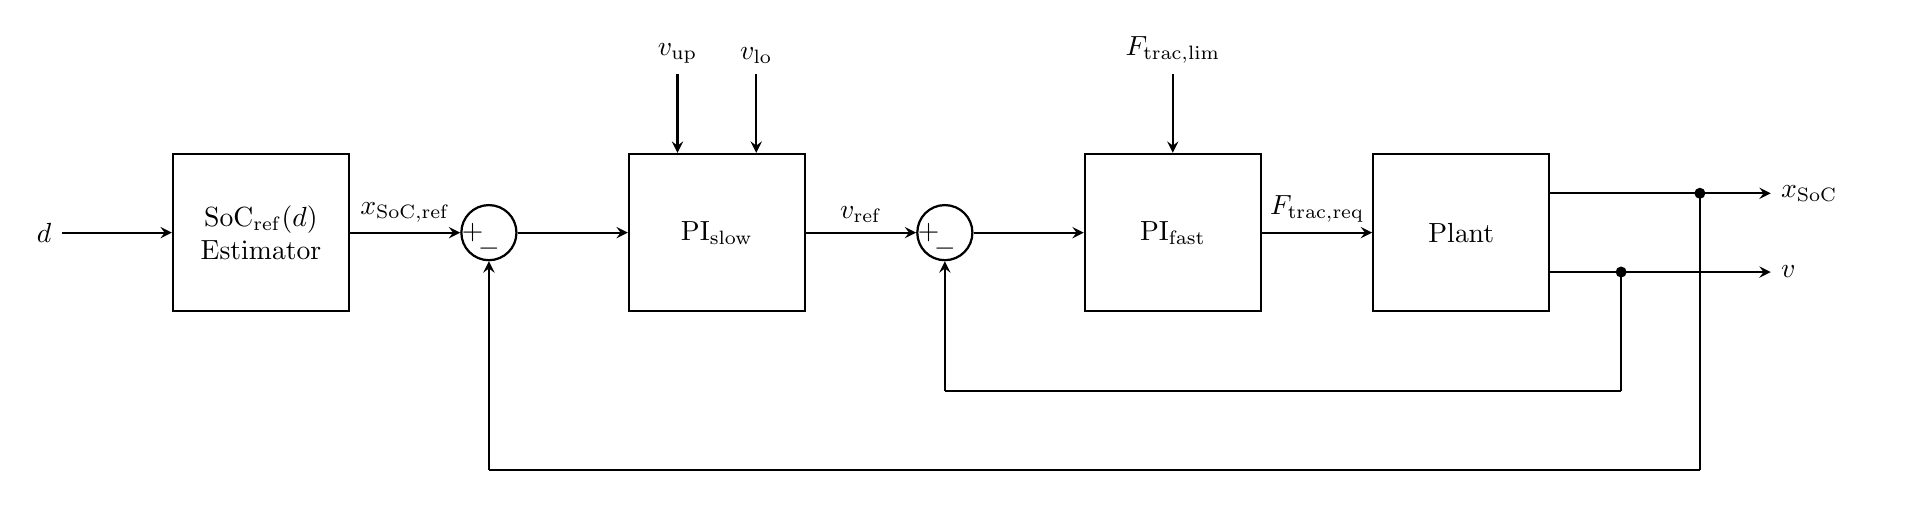
\begin{tikzpicture}
	% Definition
	%for three arrows
	\def\up{0.5}
	\def\down{-\up}
	\def\right{0.5}
	\def\left{-\right}
	%radius
	\def\radius{0.07}
	
	% Blocks
	\matrix[column sep=1.4cm, row sep=1cm]{
		%first row
		& & & \coordinate (c14); & &  \coordinate (c16); & & & &
		\\
		%second row
		\coordinate (c21); & \node[midBlock] (SoCref) {SoC$_\mathrm{ref}(d)$ \\ Estimator}; & \node[sum] (sumSoC) {}; & \node[midBlock] (Cslow) {PI$_\mathrm{slow}$}; & \node[sum] (sumVel) {}; &  \node[midBlock] (Cfast) {PI$_\mathrm{fast}$}; & \node[midBlock] (plant) {Plant}; & \coordinate (c28); & \coordinate (c29); &
		\\
		%third row
		& & & & \coordinate (c35); &  & & \coordinate (c38); & &
		\\
		%fourth row
		& & \coordinate (c43); & & &  & & \coordinate (c48); & &
		\\
	};
	
	% Arrows;
	%horizontal
	\draw[arrow] (c21) node[textInput] {$d$} -- (SoCref);
	\draw[arrow] (SoCref) -- (sumSoC) node[midway, above] {$x_\mathrm{SoC,ref}$};
	\draw[arrow] (sumSoC) -- (Cslow);
	\draw[arrow] (Cslow) -- (sumVel) node[midway, above] {$v_\mathrm{ref}$};
	\draw[arrow] (sumVel) -- (Cfast);
	\draw[arrow] (Cfast) -- (plant) node[midway, above] {$F_\mathrm{trac,req}$};
	\draw[arrow] ([yshift=\up cm]plant.east) -- ([yshift=\up cm]c29) node[textOutput] {$x_\mathrm{SoC}$};
	\draw[arrow] ([yshift=\down cm]plant.east) -- ([yshift=\down cm]c29) node[textOutput] {$v$};
	\draw[line] ([xshift=\left cm]c38) -- (c35);
	\draw[line] ([xshift=\right cm]c48) -- (c43);
	%vertical
	\draw[line] ([xshift=\left cm, yshift=\down cm]c28) -- ([xshift=\left cm]c38);
	\draw[line] ([xshift=\right cm, yshift=\up cm]c28) -- ([xshift=\right cm]c48);
	\draw[arrow] (c35) -- (sumVel);
	\draw[arrow] (c43) -- (sumSoC);
	\draw[arrow] (c16) node[textInput,above] {$F_\mathrm{trac,lim}$} -- (Cfast);
	\draw[arrow] ([xshift=\left cm]c14) node[textInput,above] {$v_\mathrm{up}$} -- ([xshift=\left cm]Cslow.north);
	\draw[arrow] ([xshift=\right cm]c14) node[textInput,above] {$v_\mathrm{lo}$} -- ([xshift=\right cm]Cslow.north);
	
	% Dots
	\fill [black] ([xshift=\left cm, yshift=\down cm]c28) circle (\radius cm);
	\fill [black] ([xshift=\right cm, yshift=\up cm]c28) circle (\radius cm);
	
	%sum
	\path pic at (sumSoC) {sum block={}{-}{+}{}};
	\path pic at (sumVel) {sum block={}{-}{+}{}};
	
\end{tikzpicture}
	\caption{Block diagram representation of the cascaded cruise controller.}
	\label{fig:simCascadedController}
\end{sidewaysfigure}

The slow controller receives two additional inputs that serve the purpose of limiting the velocity to appropriate values and activating the ARW.
\begin{align}
	v_\mathrm{up} &= \min (v_\mathrm{max}(d),v_\mathrm{cruise}) \\
	v_\mathrm{lo} &= \min (v_\mathrm{max}(d),v_\mathrm{cruise},v_\mathrm{min})
\end{align}
where $v_\mathrm{up}$ and $v_\mathrm{lo}$ are the upper and lower velocity bounds, $v_\mathrm{max}$ is the maximal speed limit, $v_\mathrm{min}$ is the minimal open road velocity, and $v_\mathrm{cruise}$ is the imposed maximal cruise velocity. The latter velocity is necessary to limit the maximum speed that our car can sustain. Their numerical values are listed in~\cref{tab:simParametersDriver}.
\begin{table}[htbp]
	\centering
	\caption{Modeling parameters for the Driver.}
	\label{tab:simParametersDriver}
	
	\begin{tabular}{l l r l}
		\toprule
		Parameter                       		& Symbol                & Value 	& Unit\\ 
		\midrule
		Maximal cruise velocity & $v_\mathrm{cruise}$ & 110 & \unitfrac{km}{h} \\
		Minimal open road velocity & $v_\mathrm{min}$ & 60 & \unitfrac{km}{h} \\
		Acceleration constant & $a_\mathrm{acc}$ & 0.7 & \unitfrac{m}{s$^2$} \\
		Deceleration constant & $a_\mathrm{dec}$ & -0.7 & \unitfrac{m}{s$^2$} \\
		\bottomrule
	\end{tabular}
\end{table}

\begin{table}[htbp]
	\centering
	\caption{Control parameters used in controllers of the Driver.}
	\label{tab:simParametersControllers}
	
	\begin{tabular}{l c c}
		\toprule
		& Proportional & Integral / $\unitfrac{1}{s}$ \\ 
		\midrule
		PI$_\mathrm{acc}$
		& 4000 & 80 \\
		\midrule
		PI$_\mathrm{dec}$
		& 4000 & 80 \\
		\midrule
		PI$_\mathrm{fast}$
		& 2000 & 500 \\
		\midrule
		PI$_\mathrm{slow}$
		& -1000 & 10 \\
		
		\bottomrule
	\end{tabular}
\end{table}

